\chapter{Phân tích hệ thống}

\section{Giới thiệu}
Chương này tập trung vào việc mô hình hóa các yêu cầu chức năng của hệ thống E-Learning Management System bằng ngôn ngữ mô hình hóa UML. Các biểu đồ use case, đặc tả use case chi tiết được xây dựng dựa trên kết quả khảo sát và phân tích nghiệp vụ ở Chương 1. Những phân tích này là cơ sở để thiết kế hệ thống ở Chương 3.

\section{Mô hình hóa chức năng}

\subsection{Biểu đồ use case tổng quan}
Hệ thống có ba tác nhân chính: \textbf{Admin}, \textbf{Teacher} (Giảng viên), \textbf{Student} (Học viên). Hình \ref{fig:uc_tongquan} mô tả các use case chính của toàn bộ hệ thống.

\begin{figure}[H]
\centering
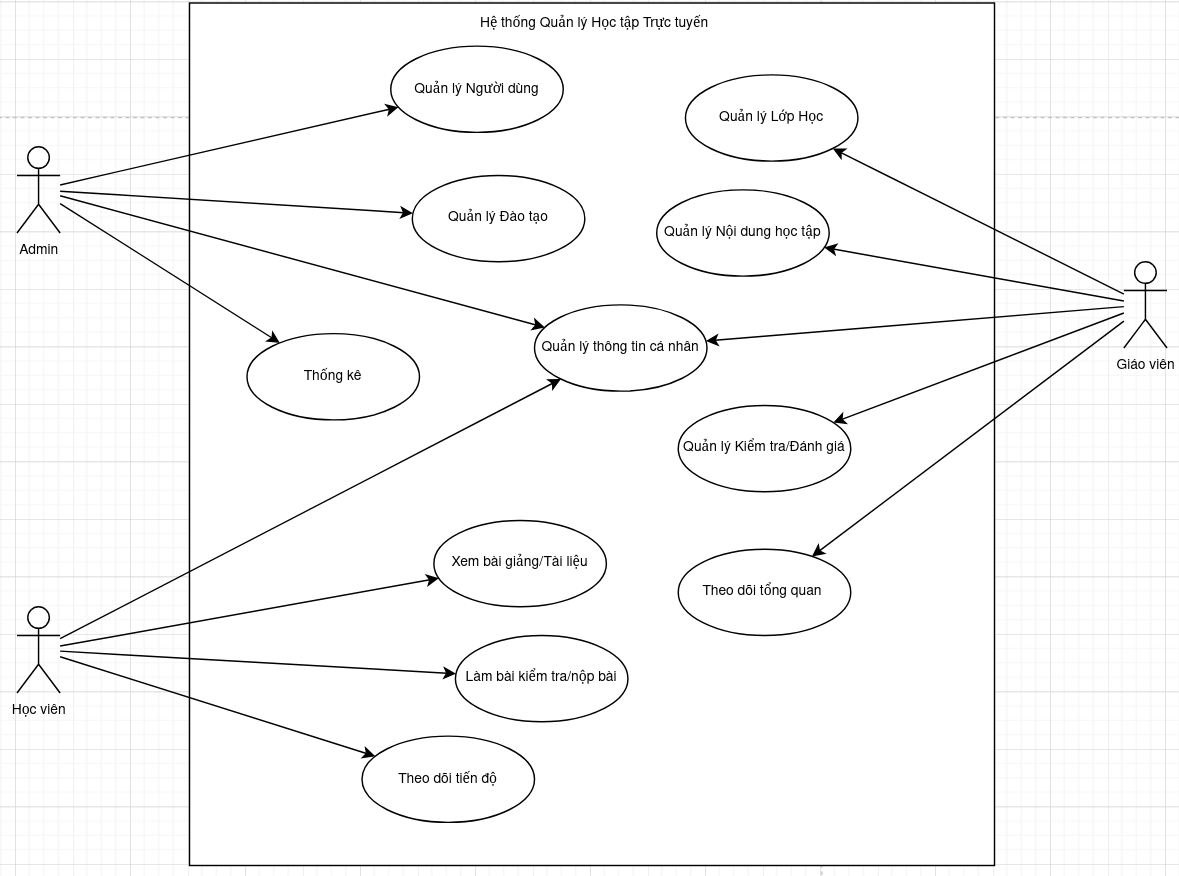
\includegraphics[width=0.9\textwidth]{figs/uc_tongquan.png}
\caption{Biểu đồ use case tổng quan hệ thống}
\label{fig:uc_tongquan}
\end{figure}

\subsection{Danh sách tác nhân (Actors)}
\begin{table}[H]
\centering
\caption{Tác nhân và mô tả}
\label{tab:actors}
\begin{tabular}{|p{3cm}|p{4cm}|p{7cm}|}
\hline
\textbf{Tác nhân} & \textbf{Ký hiệu} & \textbf{Mô tả} \\ \hline
Quản trị viên & Admin & Quản lý toàn bộ hệ thống: người dùng, khóa học, lớp học, thống kê. \\ \hline
Giảng viên & Teacher & Quản lý các lớp học được phân công, đăng tải tài liệu, bài tập, chấm điểm, theo dõi tiến độ học viên. \\ \hline
Học viên & Student & Tham gia lớp học, xem bài giảng, làm bài tập, theo dõi điểm số và tiến độ cá nhân. \\ \hline
\end{tabular}
\end{table}

\subsection{Biểu đồ use case phân rã mức 2}
Do hệ thống có nhiều chức năng, các use case chính được phân rã thành các biểu đồ con. Dưới đây là các biểu đồ phân rã cho các chức năng chính.

\begin{figure}[H]
\centering
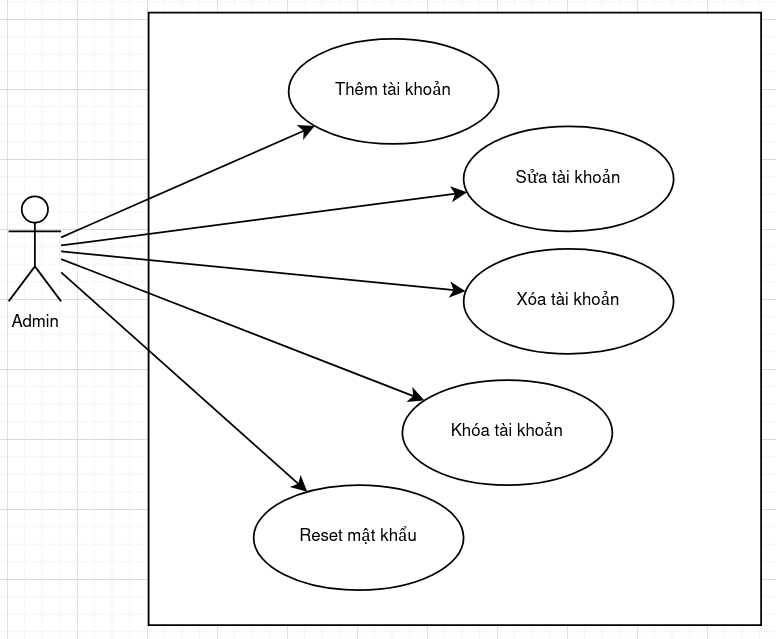
\includegraphics[width=0.8\textwidth]{figs/uc_quanlynguoidung.png}
\caption{Phân rã use case "Quản lý người dùng"}
\label{fig:uc_user}
\end{figure}

\begin{figure}[H]
\centering
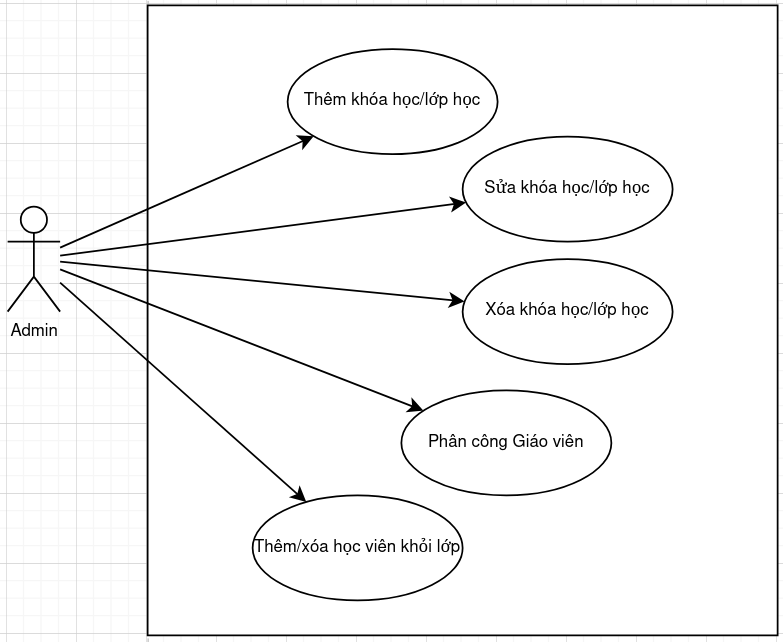
\includegraphics[width=0.8\textwidth]{figs/uc_quanlydaotao.png}
\caption{Phân rã use case "Quản lý đào tạo"}
\label{fig:uc_training}
\end{figure}

\begin{figure}[H]
\centering
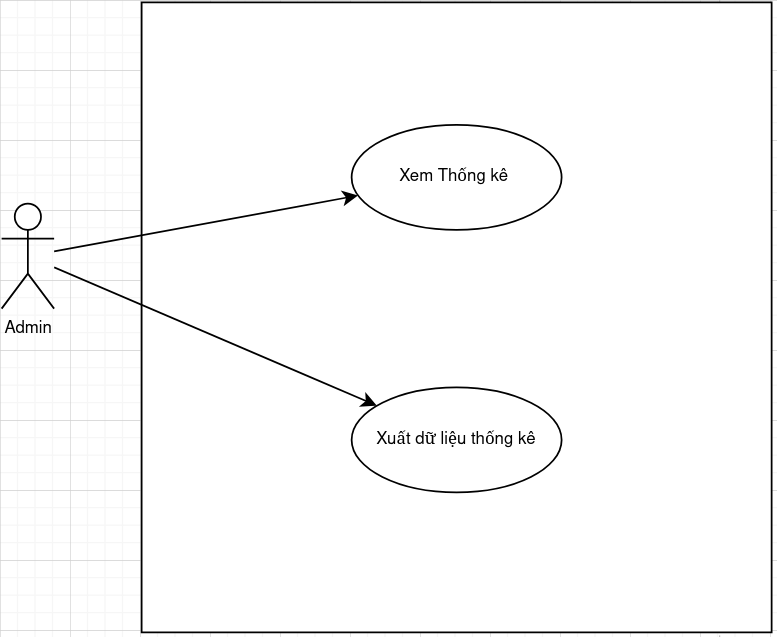
\includegraphics[width=0.8\textwidth]{figs/uc_thongke.png}
\caption{Phân rã use case "Thống kê"}
\label{fig:uc_stats}
\end{figure}

\begin{figure}[H]
\centering
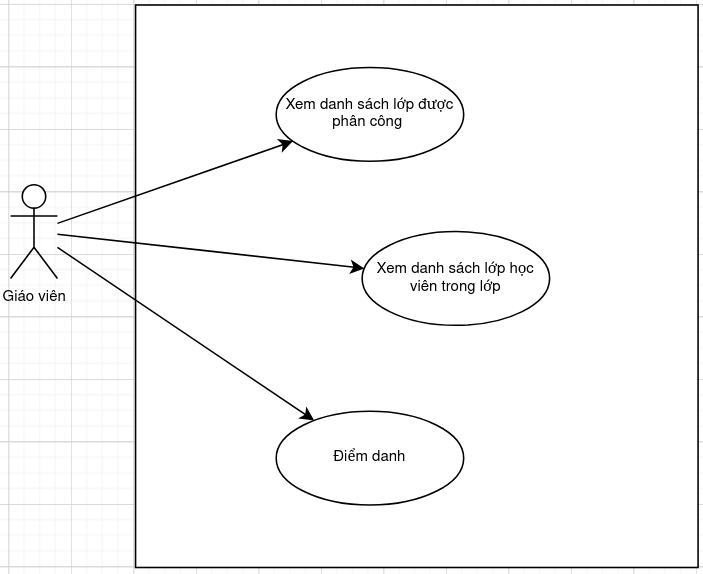
\includegraphics[width=0.8\textwidth]{figs/uc_quanlylophoc.png}
\caption{Phân rã use case "Quản lý lớp học"}
\label{fig:uc_class}
\end{figure}

\begin{figure}[H]
\centering
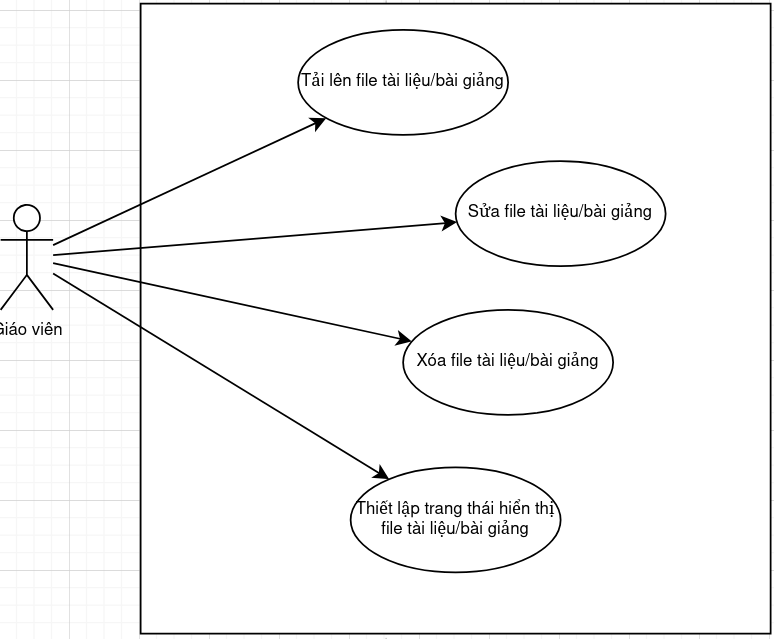
\includegraphics[width=0.8\textwidth]{figs/uc_quanlynoidung.png}
\caption{Phân rã use case "Quản lý nội dung học tập"}
\label{fig:uc_content}
\end{figure}

\begin{figure}[H]
\centering
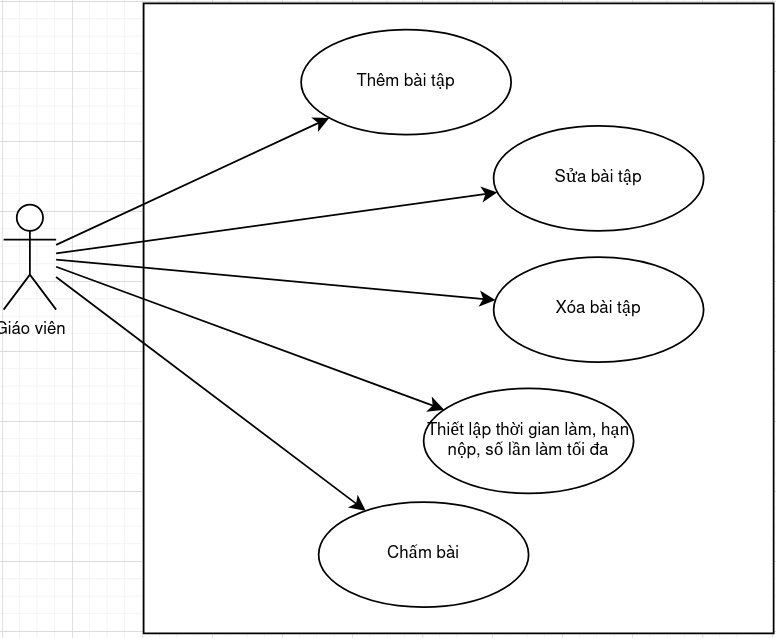
\includegraphics[width=0.8\textwidth]{figs/uc_quanlykiemtra.png}
\caption{Phân rã use case "Quản lý kiểm tra/đánh giá"}
\label{fig:uc_assessment}
\end{figure}

\begin{figure}[H]
\centering
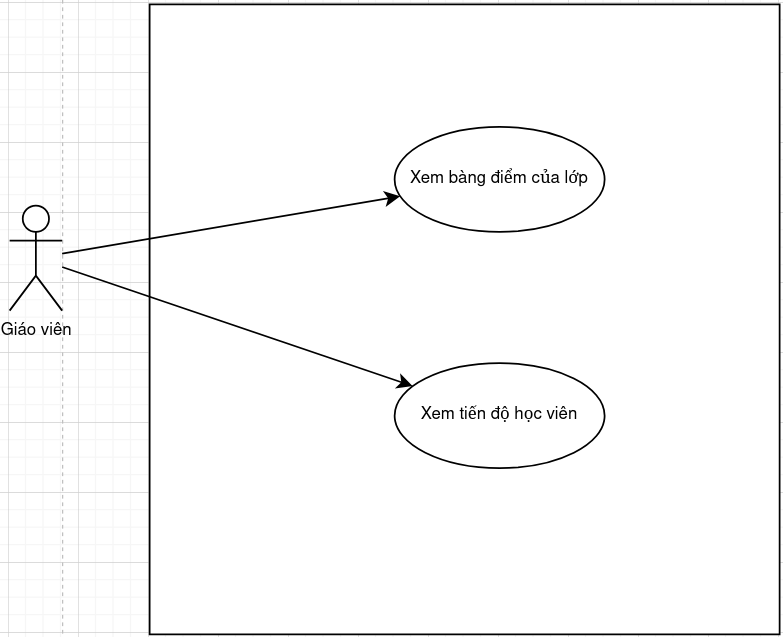
\includegraphics[width=0.8\textwidth]{figs/uc_theodoidanhgia.png}
\caption{Phân rã use case "Theo dõi tổng quan"}
\label{fig:uc_monitor}
\end{figure}

\subsection{Đặc tả use case chi tiết}
Dưới đây là đặc tả chi tiết cho 27 use case của hệ thống, bao gồm các use case của Admin, Teacher và Student.

% =================== UC001 ===================
\begin{table}[H]
\centering
\caption{UC001 – Thêm tài khoản}
\begin{tabular}{|p{2.5cm}|p{11cm}|}
\hline
\textbf{Mã UC} & UC001 \\ \hline
\textbf{Tên UC} & Thêm tài khoản \\ \hline
\textbf{Tác nhân} & Admin \\ \hline
\textbf{Mô tả} & Admin tạo mới một tài khoản cho giáo viên hoặc học viên. \\ \hline
\textbf{Tiền điều kiện} & Admin đã đăng nhập thành công. \\ \hline
\textbf{Luồng sự kiện chính} & 
\begin{minipage}{\linewidth}
\begin{enumerate}[leftmargin=*, nosep]
    \item Admin chọn mục "Quản lý người dùng" và nhấn "Thêm tài khoản mới".
    \item Hệ thống hiển thị biểu mẫu nhập thông tin (họ tên, email, mật khẩu, vai trò).
    \item Admin nhập đầy đủ thông tin hợp lệ và nhấn "Lưu".
    \item Hệ thống lưu tài khoản vào CSDL, thông báo "Thêm thành công".
\end{enumerate}
\end{minipage} \\ \hline
\textbf{Luồng thay thế} & 
\begin{minipage}{\linewidth}
\begin{itemize}[leftmargin=*, nosep]
    \item 3a. Nếu bỏ trống trường bắt buộc, hệ thống báo "Vui lòng nhập đầy đủ".
    \item 3b. Nếu email đã tồn tại, hệ thống báo "Email đã được sử dụng".
\end{itemize}
\end{minipage} \\ \hline
\end{tabular}
\end{table}

% =================== UC002 ===================
\begin{table}[H]
\centering
\caption{UC002 – Sửa tài khoản}
\begin{tabular}{|p{2.5cm}|p{11cm}|}
\hline
\textbf{Mã UC} & UC002 \\ \hline
\textbf{Tên UC} & Sửa tài khoản \\ \hline
\textbf{Tác nhân} & Admin \\ \hline
\textbf{Mô tả} & Admin cập nhật thông tin tài khoản đã tồn tại. \\ \hline
\textbf{Tiền điều kiện} & Admin đã đăng nhập; tài khoản cần sửa tồn tại. \\ \hline
\textbf{Luồng sự kiện chính} & 
\begin{minipage}{\linewidth}
\begin{enumerate}[leftmargin=*, nosep]
    \item Truy cập "Quản lý người dùng", tìm tài khoản.
    \item Nhấn nút "Sửa".
    \item Hệ thống hiển thị biểu mẫu thông tin hiện tại.
    \item Admin sửa thông tin và nhấn "Cập nhật".
    \item Hệ thống lưu thay đổi, thông báo thành công.
\end{enumerate}
\end{minipage} \\ \hline
\textbf{Luồng thay thế} & 
\begin{minipage}{\linewidth}
\begin{itemize}[leftmargin=*, nosep]
    \item 4a. Nếu bỏ trống trường bắt buộc, hệ thống báo lỗi.
\end{itemize}
\end{minipage} \\ \hline
\end{tabular}
\end{table}

% =================== UC003 ===================
\begin{table}[H]
\centering
\caption{UC003 – Xóa tài khoản}
\begin{tabular}{|p{2.5cm}|p{11cm}|}
\hline
\textbf{Mã UC} & UC003 \\ \hline
\textbf{Tên UC} & Xóa tài khoản \\ \hline
\textbf{Tác nhân} & Admin \\ \hline
\textbf{Mô tả} & Admin xóa vĩnh viễn một tài khoản. \\ \hline
\textbf{Tiền điều kiện} & Admin đã đăng nhập; tài khoản cần xóa tồn tại. \\ \hline
\textbf{Luồng sự kiện chính} & 
\begin{minipage}{\linewidth}
\begin{enumerate}[leftmargin=*, nosep]
    \item Truy cập "Quản lý người dùng", chọn tài khoản.
    \item Nhấn nút "Xóa".
    \item Hệ thống hiển thị hộp thoại xác nhận.
    \item Admin nhấn "Xác nhận".
    \item Hệ thống xóa bản ghi, cập nhật danh sách.
\end{enumerate}
\end{minipage} \\ \hline
\textbf{Luồng thay thế} & 
\begin{minipage}{\linewidth}
\begin{itemize}[leftmargin=*, nosep]
    \item 4a. Nếu Admin nhấn "Hủy", không xóa.
    \item 4b. Nếu tài khoản có dữ liệu ràng buộc, hệ thống báo lỗi.
\end{itemize}
\end{minipage} \\ \hline
\end{tabular}
\end{table}

% =================== UC004 ===================
\begin{table}[H]
\centering
\caption{UC004 – Khóa tài khoản}
\begin{tabular}{|p{2.5cm}|p{11cm}|}
\hline
\textbf{Mã UC} & UC004 \\ \hline
\textbf{Tên UC} & Khóa tài khoản \\ \hline
\textbf{Tác nhân} & Admin \\ \hline
\textbf{Mô tả} & Admin vô hiệu hóa tài khoản (tạm ngưng). \\ \hline
\textbf{Tiền điều kiện} & Admin đã đăng nhập; tài khoản đang hoạt động. \\ \hline
\textbf{Luồng sự kiện chính} & 
\begin{minipage}{\linewidth}
\begin{enumerate}[leftmargin=*, nosep]
    \item Truy cập "Quản lý người dùng", chọn tài khoản.
    \item Nhấn nút "Khóa".
    \item Hệ thống xác nhận.
    \item Admin nhấn "Xác nhận".
    \item Hệ thống cập nhật trạng thái thành "Đã khóa".
\end{enumerate}
\end{minipage} \\ \hline
\textbf{Luồng thay thế} & Nhấn "Hủy" thì giữ nguyên. \\ \hline
\end{tabular}
\end{table}

% =================== UC005 ===================
\begin{table}[H]
\centering
\caption{UC005 – Reset mật khẩu}
\begin{tabular}{|p{2.5cm}|p{11cm}|}
\hline
\textbf{Mã UC} & UC005 \\ \hline
\textbf{Tên UC} & Reset mật khẩu \\ \hline
\textbf{Tác nhân} & Admin \\ \hline
\textbf{Mô tả} & Admin đặt lại mật khẩu mặc định cho tài khoản. \\ \hline
\textbf{Tiền điều kiện} & Admin đã đăng nhập. \\ \hline
\textbf{Luồng sự kiện chính} & 
\begin{minipage}{\linewidth}
\begin{enumerate}[leftmargin=*, nosep]
    \item Truy cập "Quản lý người dùng", chọn tài khoản.
    \item Nhấn "Reset mật khẩu".
    \item Hệ thống xác nhận.
    \item Admin nhấn "Xác nhận".
    \item Hệ thống đổi mật khẩu (đã hash) và thông báo.
\end{enumerate}
\end{minipage} \\ \hline
\textbf{Luồng thay thế} & Nếu nhấn "Hủy", giữ nguyên mật khẩu cũ. \\ \hline
\end{tabular}
\end{table}

% =================== UC006 ===================
\begin{table}[H]
\centering
\caption{UC006 – Thêm khóa học/lớp học}
\begin{tabular}{|p{2.5cm}|p{11cm}|}
\hline
\textbf{Mã UC} & UC006 \\ \hline
\textbf{Tên UC} & Thêm khóa học/lớp học \\ \hline
\textbf{Tác nhân} & Admin \\ \hline
\textbf{Mô tả} & Admin tạo mới khóa học hoặc lớp học. \\ \hline
\textbf{Tiền điều kiện} & Admin đã đăng nhập. \\ \hline
\textbf{Luồng chính} & 
\begin{minipage}{\linewidth}
\begin{enumerate}[leftmargin=*, nosep]
    \item Vào "Quản lý Đào tạo" → "Thêm mới".
    \item Hiển thị biểu mẫu (tên, mô tả, lịch học, sĩ số...).
    \item Admin nhập thông tin và nhấn "Lưu".
    \item Hệ thống lưu vào CSDL, thông báo thành công.
\end{enumerate}
\end{minipage} \\ \hline
\textbf{Luồng thay thế} & 
\begin{minipage}{\linewidth}
\begin{itemize}[leftmargin=*, nosep]
    \item 3a. Thiếu thông tin bắt buộc → báo lỗi.
    \item 3b. Tên trùng → báo lỗi.
\end{itemize}
\end{minipage} \\ \hline
\end{tabular}
\end{table}

% =================== UC007 ===================
\begin{table}[H]
\centering
\caption{UC007 – Sửa khóa học/lớp học}
\begin{tabular}{|p{2.5cm}|p{11cm}|}
\hline
\textbf{Mã UC} & UC007 \\ \hline
\textbf{Tên UC} & Sửa khóa học/lớp học \\ \hline
\textbf{Tác nhân} & Admin \\ \hline
\textbf{Mô tả} & Cập nhật thông tin khóa học/lớp học. \\ \hline
\textbf{Tiền điều kiện} & Khóa học/lớp học tồn tại. \\ \hline
\textbf{Luồng chính} & 
\begin{minipage}{\linewidth}
\begin{enumerate}[leftmargin=*, nosep]
    \item Tìm mục cần sửa → nhấn "Sửa".
    \item Hệ thống hiển thị biểu mẫu hiện tại.
    \item Admin thay đổi thông tin → nhấn "Cập nhật".
    \item Lưu thay đổi, thông báo thành công.
\end{enumerate}
\end{minipage} \\ \hline
\textbf{Luồng thay thế} & Nếu sĩ số tối đa < sĩ số hiện tại → báo lỗi. \\ \hline
\end{tabular}
\end{table}

% =================== UC008 ===================
\begin{table}[H]
\centering
\caption{UC008 – Xóa khóa học/lớp học}
\begin{tabular}{|p{2.5cm}|p{11cm}|}
\hline
\textbf{Mã UC} & UC008 \\ \hline
\textbf{Tên UC} & Xóa khóa học/lớp học \\ \hline
\textbf{Tác nhân} & Admin \\ \hline
\textbf{Mô tả} & Xóa vĩnh viễn khóa học/lớp học. \\ \hline
\textbf{Tiền điều kiện} & Đối tượng cần xóa tồn tại. \\ \hline
\textbf{Luồng chính} & 
\begin{minipage}{\linewidth}
\begin{enumerate}[leftmargin=*, nosep]
    \item Chọn mục → nhấn "Xóa".
    \item Xác nhận.
    \item Hệ thống xóa dữ liệu, thông báo thành công.
\end{enumerate}
\end{minipage} \\ \hline
\textbf{Luồng thay thế} & Nếu có dữ liệu ràng buộc (lớp có học viên) → báo lỗi, không xóa. \\ \hline
\end{tabular}
\end{table}

% =================== UC009 ===================
\begin{table}[H]
\centering
\caption{UC009 – Phân công Giáo viên}
\begin{tabular}{|p{2.5cm}|p{11cm}|}
\hline
\textbf{Mã UC} & UC009 \\ \hline
\textbf{Tên UC} & Phân công Giáo viên \\ \hline
\textbf{Tác nhân} & Admin \\ \hline
\textbf{Mô tả} & Chỉ định giáo viên phụ trách lớp học. \\ \hline
\textbf{Tiền điều kiện} & Lớp học và tài khoản giáo viên đã có. \\ \hline
\textbf{Luồng chính} & 
\begin{minipage}{\linewidth}
\begin{enumerate}[leftmargin=*, nosep]
    \item Vào chi tiết lớp → "Giáo viên phụ trách".
    \item Nhấn "Thêm giáo viên".
    \item Chọn giáo viên từ danh sách → "Lưu".
    \item Hệ thống ghi nhận phân công, thông báo thành công.
\end{enumerate}
\end{minipage} \\ \hline
\textbf{Luồng thay thế} & Nếu giáo viên đã được phân công → ẩn hoặc báo lỗi. \\ \hline
\end{tabular}
\end{table}

% =================== UC010 ===================
\begin{table}[H]
\centering
\caption{UC010 – Thêm/Xóa học viên khỏi lớp}
\begin{tabular}{|p{2.5cm}|p{11cm}|}
\hline
\textbf{Mã UC} & UC010 \\ \hline
\textbf{Tên UC} & Thêm/Xóa học viên khỏi lớp \\ \hline
\textbf{Tác nhân} & Admin \\ \hline
\textbf{Mô tả} & Ghi danh hoặc xóa học viên khỏi lớp. \\ \hline
\textbf{Tiền điều kiện} & Lớp học tồn tại, học viên có tài khoản. \\ \hline
\textbf{Luồng chính} & 
\begin{minipage}{\linewidth}
\begin{enumerate}[leftmargin=*, nosep]
    \item Vào chi tiết lớp → "Danh sách học viên".
    \item Chọn "Thêm học viên" (chọn từ danh sách) hoặc "Xóa".
    \item Xác nhận.
    \item Cập nhật danh sách, thông báo.
\end{enumerate}
\end{minipage} \\ \hline
\textbf{Luồng thay thế} & 
\begin{minipage}{\linewidth}
- Nếu lớp đã đầy → không thêm được.\\
- Nếu xóa học viên đã có điểm → cảnh báo.
\end{minipage} \\ \hline
\end{tabular}
\end{table}

% =================== UC011 ===================
\begin{table}[H]
\centering
\caption{UC011 – Xem thống kê}
\begin{tabular}{|p{2.5cm}|p{11cm}|}
\hline
\textbf{Mã UC} & UC011 \\ \hline
\textbf{Tên UC} & Xem thống kê \\ \hline
\textbf{Tác nhân} & Admin \\ \hline
\textbf{Mô tả} & Xem biểu đồ, số liệu tổng quan hệ thống. \\ \hline
\textbf{Tiền điều kiện} & Admin đã đăng nhập. \\ \hline
\textbf{Luồng chính} & 
\begin{minipage}{\linewidth}
\begin{enumerate}[leftmargin=*, nosep]
    \item Vào menu "Thống kê".
    \item Hệ thống truy xuất dữ liệu.
    \item Hiển thị dưới dạng biểu đồ và card.
\end{enumerate}
\end{minipage} \\ \hline
\end{tabular}
\end{table}

% =================== UC012 ===================
\begin{table}[H]
\centering
\caption{UC012 – Xuất dữ liệu thống kê}
\begin{tabular}{|p{2.5cm}|p{11cm}|}
\hline
\textbf{Mã UC} & UC012 \\ \hline
\textbf{Tên UC} & Xuất dữ liệu thống kê \\ \hline
\textbf{Tác nhân} & Admin \\ \hline
\textbf{Mô tả} & Tải báo cáo dạng file (Excel/CSV). \\ \hline
\textbf{Tiền điều kiện} & Admin đang ở trang thống kê. \\ \hline
\textbf{Luồng chính} & 
\begin{minipage}{\linewidth}
\begin{enumerate}[leftmargin=*, nosep]
    \item Chọn bộ lọc → nhấn "Xuất file".
    \item Hệ thống tổng hợp dữ liệu, tạo file.
    \item Trình duyệt tải file về.
\end{enumerate}
\end{minipage} \\ \hline
\textbf{Luồng thay thế} & Nếu không có dữ liệu → thông báo lỗi. \\ \hline
\end{tabular}
\end{table}

% =================== UC013 ===================
\begin{table}[H]
\centering
\caption{UC013 – Xem danh sách lớp được phân công}
\begin{tabular}{|p{2.5cm}|p{11cm}|}
\hline
\textbf{Mã UC} & UC013 \\ \hline
\textbf{Tên UC} & Xem danh sách lớp được phân công \\ \hline
\textbf{Tác nhân} & Giảng viên \\ \hline
\textbf{Mô tả} & Giảng viên xem các lớp mình phụ trách. \\ \hline
\textbf{Tiền điều kiện} & Giảng viên đã đăng nhập. \\ \hline
\textbf{Luồng chính} & 
\begin{minipage}{\linewidth}
\begin{enumerate}[leftmargin=*, nosep]
    \item Vào "Lớp học của tôi".
    \item Hệ thống truy vấn dữ liệu.
    \item Hiển thị danh sách lớp.
\end{enumerate}
\end{minipage} \\ \hline
\textbf{Luồng thay thế} & Nếu chưa có lớp → thông báo trống. \\ \hline
\end{tabular}
\end{table}

% =================== UC014 ===================
\begin{table}[H]
\centering
\caption{UC014 – Xem danh sách học viên trong lớp}
\begin{tabular}{|p{2.5cm}|p{11cm}|}
\hline
\textbf{Mã UC} & UC014 \\ \hline
\textbf{Tên UC} & Xem danh sách học viên trong lớp \\ \hline
\textbf{Tác nhân} & Giảng viên \\ \hline
\textbf{Mô tả} & Xem thông tin học viên của một lớp cụ thể. \\ \hline
\textbf{Tiền điều kiện} & Giảng viên đã chọn lớp. \\ \hline
\textbf{Luồng chính} & 
\begin{minipage}{\linewidth}
\begin{enumerate}[leftmargin=*, nosep]
    \item Vào tab "Danh sách học viên".
    \item Hệ thống hiển thị danh sách.
\end{enumerate}
\end{minipage} \\ \hline
\end{tabular}
\end{table}

% =================== UC015 ===================
\begin{table}[H]
\centering
\caption{UC015 – Điểm danh}
\begin{tabular}{|p{2.5cm}|p{11cm}|}
\hline
\textbf{Mã UC} & UC015 \\ \hline
\textbf{Tên UC} & Điểm danh \\ \hline
\textbf{Tác nhân} & Giảng viên \\ \hline
\textbf{Mô tả} & Ghi nhận trạng thái có mặt/vắng của học viên. \\ \hline
\textbf{Tiền điều kiện} & Đang ở trang chi tiết lớp. \\ \hline
\textbf{Luồng chính} & 
\begin{minipage}{\linewidth}
\begin{enumerate}[leftmargin=*, nosep]
    \item Chọn "Điểm danh" → chọn buổi học.
    \item Hiển thị danh sách học viên kèm trạng thái.
    \item Giảng viên chọn trạng thái → nhấn "Lưu".
    \item Hệ thống lưu dữ liệu, thông báo.
\end{enumerate}
\end{minipage} \\ \hline
\textbf{Luồng thay thế} & Có thể chỉnh sửa lại điểm danh của buổi trước. \\ \hline
\end{tabular}
\end{table}

% =================== UC016 ===================
\begin{table}[H]
\centering
\caption{UC016 – Tải lên file tài liệu/bài giảng}
\begin{tabular}{|p{2.5cm}|p{11cm}|}
\hline
\textbf{Mã UC} & UC016 \\ \hline
\textbf{Tên UC} & Tải lên file tài liệu/bài giảng \\ \hline
\textbf{Tác nhân} & Giảng viên \\ \hline
\textbf{Mô tả} & Thêm tệp tin (PDF, Word, video) làm học liệu. \\ \hline
\textbf{Tiền điều kiện} & Giảng viên đã đăng nhập, đang ở trang quản lý lớp. \\ \hline
\textbf{Luồng chính} & 
\begin{minipage}{\linewidth}
\begin{enumerate}[leftmargin=*, nosep]
    \item Vào "Nội dung học tập" → "Tải lên tài liệu".
    \item Hiển thị biểu mẫu (tên, mô tả, chọn file).
    \item Giảng viên nhập thông tin, chọn file → "Lưu".
    \item Hệ thống lưu file lên Cloudinary, ghi đường dẫn, thông báo thành công.
\end{enumerate}
\end{minipage} \\ \hline
\textbf{Luồng thay thế} & Nếu file vượt dung lượng hoặc sai định dạng → báo lỗi. \\ \hline
\end{tabular}
\end{table}

% =================== UC017 ===================
\begin{table}[H]
\centering
\caption{UC017 – Sửa file tài liệu/bài giảng}
\begin{tabular}{|p{2.5cm}|p{11cm}|}
\hline
\textbf{Mã UC} & UC017 \\ \hline
\textbf{Tên UC} & Sửa file tài liệu/bài giảng \\ \hline
\textbf{Tác nhân} & Giảng viên \\ \hline
\textbf{Mô tả} & Cập nhật thông tin hoặc thay thế file cũ. \\ \hline
\textbf{Tiền điều kiện} & Tài liệu đã tồn tại. \\ \hline
\textbf{Luồng chính} & 
\begin{minipage}{\linewidth}
\begin{enumerate}[leftmargin=*, nosep]
    \item Tìm tài liệu cần sửa → nhấn "Sửa".
    \item Hệ thống hiển thị biểu mẫu với dữ liệu cũ.
    \item Giảng viên sửa thông tin hoặc chọn file mới → "Cập nhật".
    \item Lưu thay đổi, cập nhật file trên Cloud, thông báo thành công.
\end{enumerate}
\end{minipage} \\ \hline
\textbf{Luồng thay thế} & File mới không hợp lệ → báo lỗi. \\ \hline
\end{tabular}
\end{table}

% =================== UC018 ===================
\begin{table}[H]
\centering
\caption{UC018 – Xóa file tài liệu/bài giảng}
\begin{tabular}{|p{2.5cm}|p{11cm}|}
\hline
\textbf{Mã UC} & UC018 \\ \hline
\textbf{Tên UC} & Xóa file tài liệu/bài giảng \\ \hline
\textbf{Tác nhân} & Giảng viên \\ \hline
\textbf{Mô tả} & Gỡ bỏ tài liệu khỏi hệ thống. \\ \hline
\textbf{Tiền điều kiện} & Tài liệu tồn tại. \\ \hline
\textbf{Luồng chính} & 
\begin{minipage}{\linewidth}
\begin{enumerate}[leftmargin=*, nosep]
    \item Nhấn nút "Xóa" (thùng rác) cạnh tài liệu.
    \item Xác nhận.
    \item Hệ thống xóa bản ghi và file vật lý, thông báo.
\end{enumerate}
\end{minipage} \\ \hline
\end{tabular}
\end{table}

% =================== UC019 ===================
\begin{table}[H]
\centering
\caption{UC019 – Thiết lập trạng thái hiển thị file}
\begin{tabular}{|p{2.5cm}|p{11cm}|}
\hline
\textbf{Mã UC} & UC019 \\ \hline
\textbf{Tên UC} & Thiết lập trạng thái hiển thị file \\ \hline
\textbf{Tác nhân} & Giảng viên \\ \hline
\textbf{Mô tả} & Bật/tắt công khai tài liệu (Ẩn / Công khai). \\ \hline
\textbf{Tiền điều kiện} & Tài liệu đã tồn tại. \\ \hline
\textbf{Luồng chính} & 
\begin{minipage}{\linewidth}
\begin{enumerate}[leftmargin=*, nosep]
    \item Trong danh sách tài liệu, nhấn vào công tắc trạng thái.
    \item Hệ thống cập nhật ngay trường "status" trong CSDL.
    \item Hiển thị thông báo "Đã cập nhật trạng thái".
\end{enumerate}
\end{minipage} \\ \hline
\end{tabular}
\end{table}

% =================== UC020 ===================
\begin{table}[H]
\centering
\caption{UC020 – Thêm bài tập}
\begin{tabular}{|p{2.5cm}|p{11cm}|}
\hline
\textbf{Mã UC} & UC020 \\ \hline
\textbf{Tên UC} & Thêm bài tập \\ \hline
\textbf{Tác nhân} & Giảng viên \\ \hline
\textbf{Mô tả} & Tạo bài tập (tự luận hoặc trắc nghiệm) giao cho học viên. \\ \hline
\textbf{Tiền điều kiện} & Giảng viên đang ở không gian lớp học. \\ \hline
\textbf{Luồng chính} & 
\begin{minipage}{\linewidth}
\begin{enumerate}[leftmargin=*, nosep]
    \item Vào "Bài tập/Kiểm tra" → "Thêm bài tập mới".
    \item Hiển thị form (tiêu đề, loại, nội dung/câu hỏi).
    \item Giảng viên nhập → "Lưu".
    \item Lưu vào CSDL, hiển thị lên danh sách.
\end{enumerate}
\end{minipage} \\ \hline
\textbf{Luồng thay thế} & Nếu thiếu tiêu đề hoặc nội dung → báo lỗi. \\ \hline
\end{tabular}
\end{table}

% =================== UC021 ===================
\begin{table}[H]
\centering
\caption{UC021 – Sửa bài tập}
\begin{tabular}{|p{2.5cm}|p{11cm}|}
\hline
\textbf{Mã UC} & UC021 \\ \hline
\textbf{Tên UC} & Sửa bài tập \\ \hline
\textbf{Tác nhân} & Giảng viên \\ \hline
\textbf{Mô tả} & Cập nhật nội dung bài tập. \\ \hline
\textbf{Tiền điều kiện} & Bài tập tồn tại. \\ \hline
\textbf{Luồng chính} & 
\begin{minipage}{\linewidth}
\begin{enumerate}[leftmargin=*, nosep]
    \item Tìm bài tập → nhấn "Sửa".
    \item Hiển thị dữ liệu cũ.
    \item Giảng viên sửa → "Cập nhật".
    \item Lưu thay đổi, thông báo.
\end{enumerate}
\end{minipage} \\ \hline
\textbf{Luồng thay thế} & Nếu đã có học viên nộp bài → cảnh báo. \\ \hline
\end{tabular}
\end{table}

% =================== UC022 ===================
\begin{table}[H]
\centering
\caption{UC022 – Xóa bài tập}
\begin{tabular}{|p{2.5cm}|p{11cm}|}
\hline
\textbf{Mã UC} & UC022 \\ \hline
\textbf{Tên UC} & Xóa bài tập \\ \hline
\textbf{Tác nhân} & Giảng viên \\ \hline
\textbf{Mô tả} & Xóa bài tập khỏi hệ thống. \\ \hline
\textbf{Tiền điều kiện} & Bài tập tồn tại. \\ \hline
\textbf{Luồng chính} & 
\begin{minipage}{\linewidth}
\begin{enumerate}[leftmargin=*, nosep]
    \item Chọn bài tập → "Xóa".
    \item Xác nhận.
    \item Hệ thống xóa dữ liệu.
\end{enumerate}
\end{minipage} \\ \hline
\textbf{Luồng thay thế} & Nếu đã có học viên nộp bài → chặn xóa, yêu cầu ẩn. \\ \hline
\end{tabular}
\end{table}

% =================== UC023 ===================
\begin{table}[H]
\centering
\caption{UC023 – Thiết lập thời gian làm, hạn nộp, số lần làm tối đa}
\begin{tabular}{|p{2.5cm}|p{11cm}|}
\hline
\textbf{Mã UC} & UC023 \\ \hline
\textbf{Tên UC} & Thiết lập thời gian làm, hạn nộp, số lần làm tối đa \\ \hline
\textbf{Tác nhân} & Giảng viên \\ \hline
\textbf{Mô tả} & Cấu hình các luật cho bài tập. \\ \hline
\textbf{Tiền điều kiện} & Bài tập đã được tạo. \\ \hline
\textbf{Luồng chính} & 
\begin{minipage}{\linewidth}
\begin{enumerate}[leftmargin=*, nosep]
    \item Chọn bài tập → "Cài đặt/Cấu hình".
    \item Hiển thị biểu mẫu (thời gian làm bài, deadline, số lần nộp).
    \item Giảng viên nhập thông số → "Lưu cài đặt".
    \item Cập nhật metadata, thông báo.
\end{enumerate}
\end{minipage} \\ \hline
\textbf{Luồng thay thế} & Nếu deadline trong quá khứ → báo lỗi. \\ \hline
\end{tabular}
\end{table}

% =================== UC024 ===================
\begin{table}[H]
\centering
\caption{UC024 – Chấm bài}
\begin{tabular}{|p{2.5cm}|p{11cm}|}
\hline
\textbf{Mã UC} & UC024 \\ \hline
\textbf{Tên UC} & Chấm bài \\ \hline
\textbf{Tác nhân} & Giảng viên \\ \hline
\textbf{Mô tả} & Chấm bài tự luận, nhập điểm và nhận xét. \\ \hline
\textbf{Tiền điều kiện} & Bài tập tự luận đã có học viên nộp. \\ \hline
\textbf{Luồng chính} & 
\begin{minipage}{\linewidth}
\begin{enumerate}[leftmargin=*, nosep]
    \item Chọn bài tập → tab "Danh sách nộp bài".
    \item Hiển thị danh sách học viên và file đính kèm.
    \item Giảng viên xem file, nhập điểm, nhận xét → "Lưu điểm".
    \item Lưu vào gradebook, thông báo.
\end{enumerate}
\end{minipage} \\ \hline
\end{tabular}
\end{table}

% =================== UC025 ===================
\begin{table}[H]
\centering
\caption{UC025 – Xem bảng điểm của lớp}
\begin{tabular}{|p{2.5cm}|p{11cm}|}
\hline
\textbf{Mã UC} & UC025 \\ \hline
\textbf{Tên UC} & Xem bảng điểm của lớp \\ \hline
\textbf{Tác nhân} & Giảng viên \\ \hline
\textbf{Mô tả} & Xem tổng hợp điểm số tất cả học viên trong lớp. \\ \hline
\textbf{Tiền điều kiện} & Đang ở không gian quản lý lớp. \\ \hline
\textbf{Luồng chính} & 
\begin{minipage}{\linewidth}
\begin{enumerate}[leftmargin=*, nosep]
    \item Chọn tab "Bảng điểm" (Gradebook).
    \item Hệ thống truy xuất điểm số → hiển thị bảng.
\end{enumerate}
\end{minipage} \\ \hline
\textbf{Luồng thay thế} & Có thể xuất bảng điểm ra Excel. \\ \hline
\end{tabular}
\end{table}

% =================== UC026 ===================
\begin{table}[H]
\centering
\caption{UC026 – Xem tiến độ học viên}
\begin{tabular}{|p{2.5cm}|p{11cm}|}
\hline
\textbf{Mã UC} & UC026 \\ \hline
\textbf{Tên UC} & Xem tiến độ học viên \\ \hline
\textbf{Tác nhân} & Giảng viên \\ \hline
\textbf{Mô tả} & Theo dõi tỷ lệ hoàn thành khóa học của từng học viên. \\ \hline
\textbf{Tiền điều kiện} & Đang ở không gian quản lý lớp. \\ \hline
\textbf{Luồng chính} & 
\begin{minipage}{\linewidth}
\begin{enumerate}[leftmargin=*, nosep]
    \item Chọn tab "Tiến độ học tập".
    \item Hệ thống tính % hoàn thành → hiển thị progress bar.
\end{enumerate}
\end{minipage} \\ \hline
\end{tabular}
\end{table}

% =================== UC027 ===================
\begin{table}[H]
\centering
\caption{UC027 – Xem danh sách lớp học (Học viên)}
\begin{tabular}{|p{2.5cm}|p{11cm}|}
\hline
\textbf{Mã UC} & UC027 \\ \hline
\textbf{Tên UC} & Xem danh sách lớp học \\ \hline
\textbf{Tác nhân} & Học viên \\ \hline
\textbf{Mô tả} & Học viên xem các lớp mình đã ghi danh. \\ \hline
\textbf{Tiền điều kiện} & Học viên đã đăng nhập. \\ \hline
\textbf{Luồng chính} & 
\begin{minipage}{\linewidth}
\begin{enumerate}[leftmargin=*, nosep]
    \item Vào "Lớp học của tôi".
    \item Hệ thống truy vấn → hiển thị danh sách lớp kèm tiến độ.
\end{enumerate}
\end{minipage} \\ \hline
\textbf{Luồng thay thế} & Nếu chưa có lớp → thông báo trống. \\ \hline
\end{tabular}
\end{table}

\section{Kết luận chương}
Chương 2 đã xây dựng các biểu đồ use case (tổng quan và phân rã) cùng với bảng đặc tả chi tiết cho 27 use case của hệ thống. Các phân tích này cung cấp một cái nhìn toàn diện về các chức năng mà hệ thống cần đáp ứng, làm cơ sở vững chắc cho việc thiết kế cơ sở dữ liệu, giao diện và kiến trúc hệ thống ở Chương tiếp theo.
